\chapter{Amplifiers}

In this section, we will study amplifiers: circuits that take a signal as input and produce an identical but magnified version at the output. We'll see the basic amplifier and the more stable four-resistor version. Next, we study the most common amplifier topologies - common emitter, common base and common collector - and what are their advantages and drawbacks. Finally, we study the differential amplifier and the operational amplifier or OPAMP.


\section{Basic Amplifier}
In this section, we will develop and improve a basic amplifier. The elementary circuit we will be using is shown in figure \ref{fig:amplifier0}. Bias currents $I_{BQ}$ and $I_{CQ}$ are generated by the DC voltage source $E_B$.  The time-varying voltage source $v_i$ is the input signal, and is applied at the base of the transistor\footnote{Note that in reality this is the result of applying Thevenin's theorem to resistors $R_1$ and $R_2$}. The output is measured at the collector.\\
As $v_i$ increases, so does $i_B$, just as in figure \ref{fig:small_signal_resp6}. If the transistor is biased in the normal operating region, then $i_C = \beta i_B$ will also increase. As we move along the load line with increasing $i_C$, the voltage drop along $R_C$ increases and the output voltage $v_o$ decreases. We want to compute the voltage gain $A_v$. But before we do that, we first see how the input part of the circuit in figure \ref{fig:amplifier0} can be constructed.
\begin{figure}[h!]
	\centering
	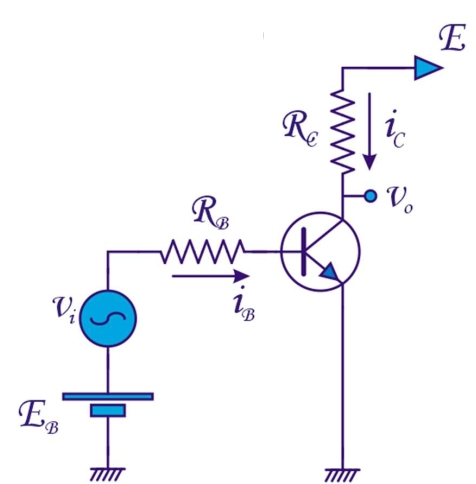
\includegraphics[width=6cm]{figures/ch02/amplifier0.jpg}
	\caption{Simple amplifier}
	\label{fig:amplifier0}
\end{figure}
\subsection{Coupling Capacitance}
Let's compute the corresponding Thevenin equivalent of the circuit in figure \ref{fig:amplifier1}. To find $e_0$, apply Millman's theorem:
\begin{equation}
	\begin{split}
		e_0 &= \frac{E/R_1 + e_i \; j\omega C_B}{1/R_1 + 1/R_2 + j\omega C_B} \\
		&= \frac{R_2 E + e_i \; j\omega C_B R_2}{R_1 + R_2 + j\omega C_B R_1 R_2} \\
		&= E \frac{R_2}{R_1+R_2}\frac{1}{1+j\omega C_B R_B} + e_i\frac{j\omega C_B R_B}{1+j\omega C_B R_B}\\
	\end{split}
	\label{eq:couplig_cap}
\end{equation}
with $R_B = \frac{R_1 R_2}{R_1 + R_2}$. If $\omega$ is much smaller than the critical pulsation $\omega_c = \frac{1}{R_B C_B}$, then $e_0 \approx  E \frac{R_2}{R_1+R_2}$. If $\omega \gg \omega_c$, then $e_0 \approx e_i$. The latter condition corresponds to assuming $C_B$ is a short-circuit.\ Another way to find equation \ref{eq:couplig_cap}, is to use the superposition principle: first, consider only $E$ with $e_i = 0$, then consider $e_i$ with $E=0$, and add both results.\\
The circuit is thus equivalent to a DC source $E_B = E \frac{R_2}{R_1+R_2}$ in series with a small-signal, high-frequency source $e_i$, just as in  figure \ref{fig:amplifier2}. This means we can use this circuit to couple $e_i$ to the input of the amplifier, while keeping the DC biasing, just as in figure \ref{fig:amplifier0}. Capacitor $C_B$ is a \emph{coupling capacitor} because it "couples" $v_i$ into the circuit.\\
\begin{minipage}{.5\textwidth}
	\centering
	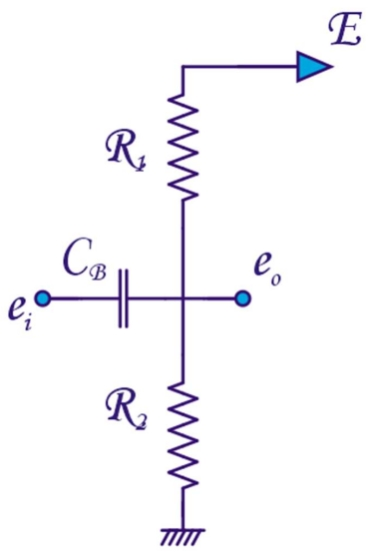
\includegraphics[width=3cm]{figures/ch02/amplifier1.jpg}
	\captionof{figure}{}
	\label{fig:amplifier1}
\end{minipage}%
\begin{minipage}{.5\textwidth}
	\centering
	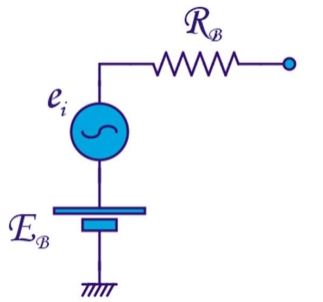
\includegraphics[width=5cm]{figures/ch02/amplifier2.jpg}
	\captionof{figure}{}
	\label{fig:amplifier2}
\end{minipage}

\subsubsection{Voltage gain $A_v$}

\begin{minipage}{.5\textwidth}
	To calculate $A_v$, we draw the small-signal equivalent circuit, by replacing the npn-transistor by its small-signal model, and by grounding the DC voltage source $E$. We also assume that the frequency we consider is higher than $\frac{1}{R_B C_B}$, so we can consider $C_B$ as a short-circuit. The small-signal circuit is shown in figure \ref{fig:amplifier3}. The parameters of the model are set by the operating currents and voltages:
\end{minipage}%
\begin{minipage}{.5\textwidth}
	\centering
	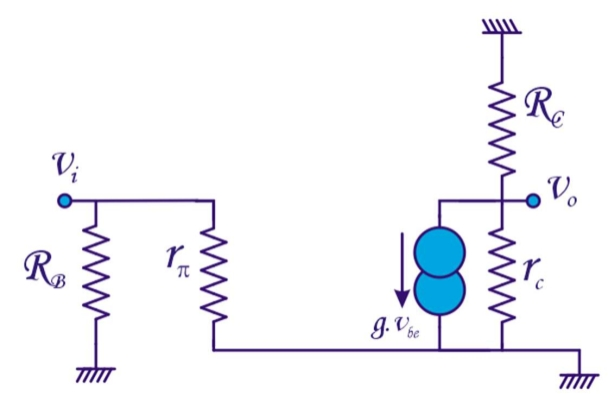
\includegraphics[width=6cm]{figures/ch02/amplifier3.jpg}
	\captionof{figure}{Amplifier - small-signal model}
	\label{fig:amplifier3}
\end{minipage}

\begin{itemize}
	\item $r_{\pi} = \frac{v_{th}}{I_{BQ}}$,
	\item $r_c = \frac{V_E}{I_{CQ}}$,
	\item $g = \frac{I_{CQ}}{v_{th}}$
\end{itemize}
In the equivalent circuit, we apply Millman in $v_o$:

$$v_o = \frac{-g \; v_{be}}{g_c +G_C}$$
and we see that $v_{be} = v_i$. As a consequence: 
\begin{equation}
	A_v = \frac{v_o}{v_i} = - g \; (r_c || R_C)
\end{equation}
For a MOSFET, we would have found a similar expression: $A_v = - g_m (r_{ds} || R_D)$. Note that the gain is negative, because an increase in $i_b$ and thus in $i_c$ will lead to a larger drop across $R_C$ and will decrease $v_o$, as explained previously.\\
The gain can be increased by:
\begin{enumerate}
	\item Increasing $g$ by setting a higher $I_{CQ}$. This will also decrease $r_c$, but this is usually not a problem since most of the times $r_c \gg R_C$ and hence $R_C || r_c \approx R_C$. In that case, $A_v \approx -g\;R_C$.
	\item Increase $R_C$. The drawback is that this decrease the potential swing of $v_o$.
\end{enumerate}
The maximum voltage gain we can obtain for a BJT is found when $R_C \rightarrow \infty$. Then is
$$A_{v,max} = -gr_c = - \frac{I_{CQ}}{v_{th}} \frac{V_E}{I_{CQ}} \approx -40 \times \frac{1}{0.026} \approx -1600$$
For a MOSFET, $A_{v,max}$ is about $-400$.
\subsection{The $4$-resistor amplifier}
\label{sec:four_resistor}
We will study a more general circuit, namely the amplifier with $4$ biasing resistors that we saw before and is reproduced in figure \ref{fig:amplifier4}(left). As before, we assume that the input frequency of interest is such that we can consider $C_B$ as a short circuit. Note that the small-signal circuit would be the same for an n-channel MOSFET, if $r_{\pi} \rightarrow \infty$.\\
\begin{figure}[h!]
	\centering
	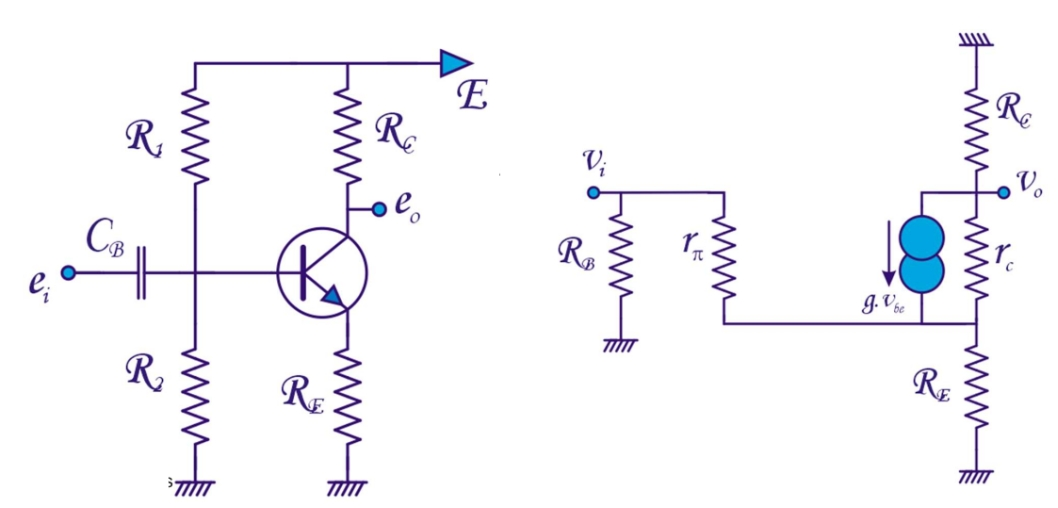
\includegraphics[width=14cm]{figures/ch02/amplifier4.jpg}
	\caption{Four-resistor amplifier (left) and small-signal equivalent circuit (right)}
	\label{fig:amplifier4}
\end{figure}
To compute $A_v$, apply Millman at both the emitter and collector (output) node:
\begin{itemize}
	\item At collector: $v_o = \frac{g_c v_e - g(v_i - v_e)}{G_c + g_c}$ because  $v_{be} = v_i - v_e$. Note that we used conductivities. For example, $G_c = 1/R_c$.
	\item At emitter: $v_e = \frac{g_{\pi} v_i g_c v_o + g(v_i - v_e)}{G_E + g_c + g_{\pi}}$
\end{itemize}
After eliminating $v_e$, we obtain:
\begin{equation}
	\begin{split}
		A_v &= \frac{-g R_C r_c r_{\pi} + R_C R_E}{(r_c + R_C)(R_E + r_{\pi}) + r_{\pi} R_E(1 + g r_c)}\\
		%			&= -\frac{r R_C r_c}{r_c + R_C + R_E(1+gr_c)} \\
		&= -g \frac{r_c R_C}{r_c + R_C} \frac{r_{\pi} - \frac{R_E}{g r_C}}{R_E + r_{\pi}(1 + R_E \frac{1+ g r_c}{r_c + R_C})} \\
		&\approx -\frac{R_C}{R_E}
	\end{split}
	\label{eq:4resistor_dc}
\end{equation}
where we assumed that $r_c \gg R_C$ and $g r_c \gg 1$.\\
It is logical that $A_v \approx -R_C/R_E$: in a first approximation, as the base voltage increases with $v_i$, the emitter voltage will follow because they are tied together by the drop across base-emitter junction, which is about $0.6$ V. If the emitter voltage increases by $v_i$, the emitter current will increase by $\frac{v_i}{R_E}$. This is also approximately the increase in collector current, thus the voltage drop increase at $R_C$ is equal to $v_o \approx -R_C \frac{v_i}{R_E}$.\\
%\textbf{TODO: add comment on phase splitter}\\
We compare this result to the version with no emitter resistance, for which $A_v \approx -g\;R_C$. We take as nominal values $R_C = 1 k\Omega$, $R_E = 500 \Omega$ and $g = 40 mA/V$. Without $R_E$, we find a gain of $40$, while with $R_E$, the gain is $2$. Thus, while $R_E$ is necessary to obtain a stable bias point, its presence significantly reduces the gain. Hence we use a bypass capacitor as in figure \ref{fig:loadline7}.
\subsubsection{Frequency analysis}
\begin{wrapfigure}{r}{0.4\textwidth}
	\centering
	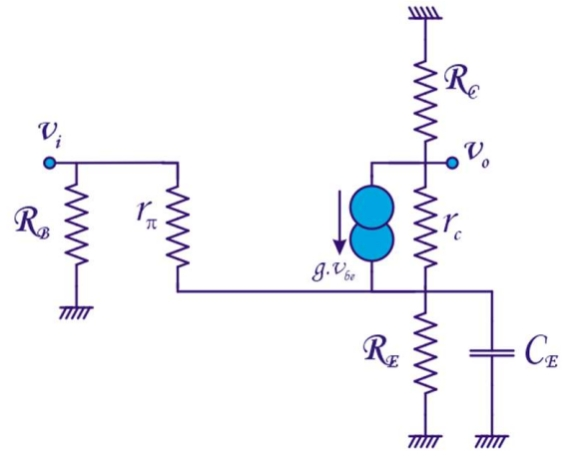
\includegraphics[width=5cm]{figures/ch02/amplifier5.jpg}
	\caption{}%$4R$ amplifier with bypass capacitance - small-signal model}
	\label{fig:amplifier5}
\end{wrapfigure}

We will study how the amplifier gain $A_v = \frac{v_o}{v_i}$ depends on frequency. To do this, we establish the small-signal circuit for the four-resistor amplifier with bypass capacitance $C_E$ and coupling capacitance $C_B$, as in figure \ref{fig:amplifier5}. The parallel combination of $R_E$ and $C_E$ gives:
\begin{equation}
	Z_E = \frac{R_E}{1 + j \omega R_E C_E}
\end{equation}
and we substitute this expression for $R_E$ in equation \ref{eq:4resistor_dc}. At the same this, we multiply by $\frac{j\omega R_B C_B}{1+j\omega R_B C_B} $, just as in equation \ref{eq:couplig_cap}. 
\begin{equation}
	A_v = \frac{j\omega R_B C_B}{1+j\omega R_B C_B} \frac{-g R_C r_c r_{\pi} + R_C Z_E}{(r_c + R_C)(Z_E + r_{\pi}) + r_{\pi} Z_E(1 + g r_c)}
\end{equation}
If we set $T_B = 1/(R_B C_B)$ and $T_E = 1/(R_E C_E)$, this equation can be simplified to:
\begin{equation}
	A_v \approx -  A_{vE} \frac{j \omega T_B}{1 + j \omega T_B} \frac{1 + j \omega T_E}{1 + j \omega T_E    \frac{A_{vE}}{A_{v0}} } 
\end{equation}
with $A_{vE} = \frac{R_C}{R_E}$ and $A_{v0} = g \frac{R_C r_c}{R_C + r_c}$. This transmittance has two poles in $\omega=1/T_B$ and $\omega = \frac{A_{v0}}{T_E \; A_{vE}}$ and zeros in $\omega=0$ and $\omega = 1/T_E$. With $A_{v0} \gg A_{vE}$ and a correct choice for $R_B C_B$ and $R_E C_E$, we have:
$$1/T_B < 1/T_E < \frac{A_{v0}}{T_E \; A_{vE}}$$
\begin{figure}[h!]
	\centering
	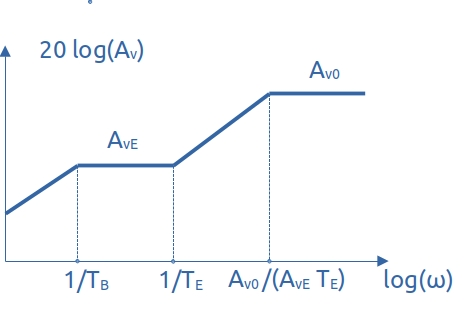
\includegraphics[width=9cm]{figures/ch02/amplifier6.jpg}
	\caption{$4R$ $A_v$ Bode Curve}
	\label{fig:amplifier6}
\end{figure}
Figure \ref{fig:amplifier6} shows the bode plot of $A_v(\omega)$. We find four different domains based on the frequency of the input signal:
\begin{enumerate}
	\item $\omega < 1/T_B$: the signal $v_i$ is not yet coupled into the base of the amplifier through capacitance $C_B$.
	\item  $1/T_B < \omega < 1/T_E$: capacitance $C_B$ can be considered as a short circuit. However, $\omega$ is to small to short-circuit $C_E$ and bypass $R_E$. The gain is thus about $-R_C/R_E$.
	\item $1/T_E < \omega < A_{v0}/(A_{vE} T_E)$: as $\omega$ increases, $R_E$ starts to get bypassed.
	\item $\omega > A_{v0}/(A_{vE} T_E)$: the maximum gain (with bypassed $R_E$) is reached: $A_{v0} = -g (R_C || r_c)$. This is the domain in which we want to use the amplifier.
\end{enumerate}
It is important to note that the critical pulsation is not $1/T_E$ but rather $\omega_{crit} = \frac{A_{v0}}{A_{vE} T_E}$. Note also that $A_{vE} \approx -\frac{R_C}{R_E}$ and $A_{v0} \approx -g\;R_C$, so the critical pulsation is $\frac{1}{T_E} \frac{A_{v0}}{A_{vE}} \approx \frac{1}{R_E C_E} \frac{g R_C}{\frac{R_C}{R_E}} = \frac{g}{C_E}$.

\newpage
\section{Basic Topologies}
\subsection{Common Emitter Amplifier (CEA)}
\label{sec:cea}
The amplifier configuration of the previous section is the \emph{common-emitter} configuration: the input is at the transistor base (gate) and the output is at the collector (drain). For the frequencies of interest, the emitter (source) is bound to ground and thus at a "common" voltage. Other configurations are the common-base and common-collector. We will study these configurations in the next sections.\\
Our goal is to establish the voltage gain, and input- and output impedances for the common-emitter configuration. For this purpose, we once again draw the small-signal equivalent circuit as in figure \ref{fig:amplifier7}.
\begin{figure}[h!]
	\centering
	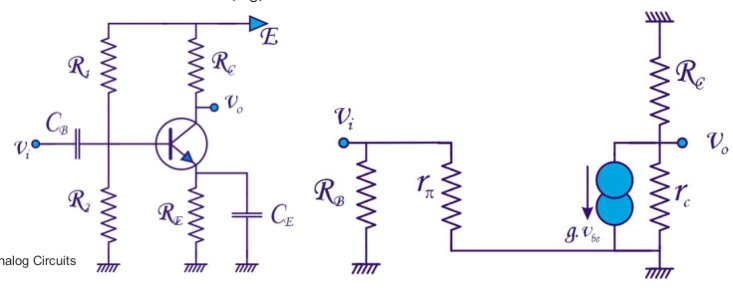
\includegraphics[width=14cm]{figures/ch02/amplifier7.jpg}
	\caption{CEA: circuit (left) and small-signal equivalent (right)}
	\label{fig:amplifier7}
\end{figure}
\begin{itemize}
	\item Voltage gain $A_v$: For an input voltage $v_i$, $v_{be} = v_i$. Thus $v_o = -g v_i (R_C || r_c)$ and $A_v = -g (R_C || r_c) = -\frac{g}{g_c + G_C}$ as we've seen before.
	\item Input impedance $Z_i = v_i/i_i = \frac{1}{g_{\pi} + G_B} = r_{\pi} || R_B$.
	\item Output impedance: to compute $Z_o$:
	\begin{itemize}
		\item Shorten $v_i$ to ground,
		\item Apply $v_o$ (or $i_o$) to the output,
		\item Compute $i_o$ (or $v_o$),
		\item The output impedance $Z_o = \frac{v_o}{i_o}$.
	\end{itemize}
	The effect of shortening the input to ground is that $v_{be} = 0$ is in figure \ref{fig:amplifier7}. Thus the current source with transconductance $g$ can be omitted. We see that then the output impedance is the parallel combination of $R_C$ and $r_c$: $Z_o = \frac{1}{G_C + g_c}$.
\end{itemize}

\subsection{Common Base Amplifier (CBA)}
\label{sec:cba}
In a common-base configuration, the base of the transistor is kept at a constant voltage (i.e. an AC ground). The input signal is applied to the emitter and the output voltage is measured at the collector. The circuit is shown in the left part of figure \ref{fig:amplifier8}, with the small-signal circuit on the right. Obviously, a bypass capacitance is not added.

\begin{figure}[h!]
	\centering
	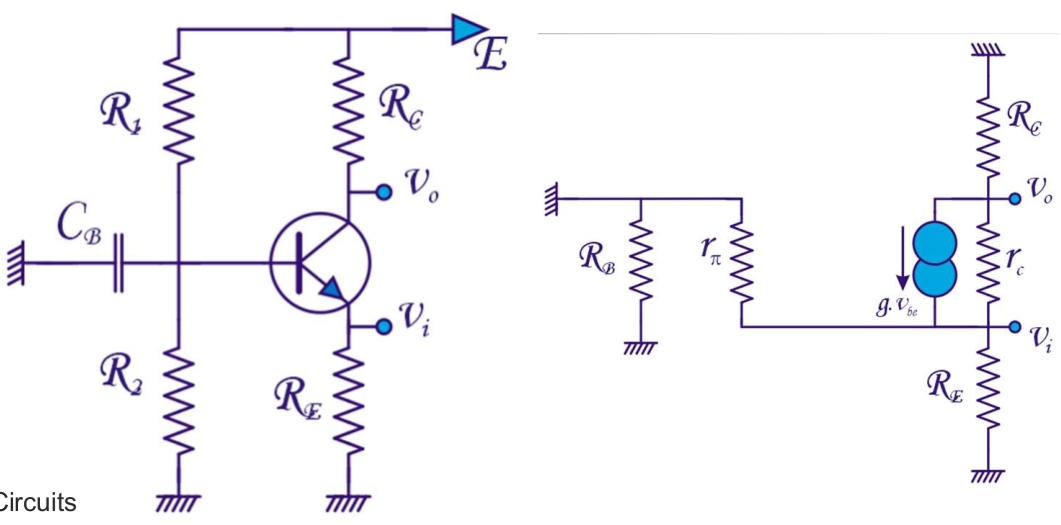
\includegraphics[width=14cm]{figures/ch02/amplifier8.jpg}
	\caption{CBA: circuit (left) and small-signal equivalent (right)}
	\label{fig:amplifier8}
\end{figure}

\begin{itemize}
	\item Voltage gain $A_v$: we see that $v_{be} = -v_i$. In the output node, we can write:
	\begin{equation}
		\begin{split}
			v_o &= \frac{g_c v_i - g (-v_i)}{G_C + g_c} \\ 
			\rightarrow A_v &= \frac{v_o}{v_i} = \frac{g + g_c}{G_C + g_c} \\
			&\approx \frac{g}{G_C + g_c} = g (R_C || r_c)
		\end{split}
	\end{equation}
	because $g \gg g_c$. Notice how the gain is positive, and the same (in absolute value) as for the common-emitter configuration. 
	\item Input impedance $Z_i$: 
\begin{comment}
	\begin{equation}
		\begin{split}
			i_i &= (G_E + g_{\pi}) v_i + G_C v_o  \\
			i_i &= (G_E + g_{\pi} + g + g_c) v_i + G_C \bigg(\frac{g + g_c}{G_C + g_c} \bigg) v_i\\
			&= \frac{(G_C + g_c)(G_E + g_{\pi} + g + g_c) + G_C(g + g_c)}{G_C + g_c}
		\end{split}
	\end{equation}
	The first expression is possible because we know that the current out of $v_i$ through $g$ and $g_c$ is equal to the current through $G_C: G_C \; v_o$. Thus:
	\begin{equation}
		\begin{split}
			\rightarrow Z_{i} &= \frac{v_i}{i_i} =  \frac{G_C + g_c} {(G_C + g_c)(G_E + g_{\pi} + g + g_c) + G_C(g + g_c)}\\
			&\approx \frac{1}{G_E + g}\\
			&\approx \frac{1}{g} \text{ if } R_E \rightarrow \infty
		\end{split}
	\end{equation}
\end{comment}
	We compute the current drawn at the input node:
	\begin{equation}
		\begin{split}
			i_i &= G_E v_i + g_{\pi} v_i + g_c (v_i - v_o) - g v_i \\
		\end{split}
	\end{equation}
	Substituting the expression for $v_o$: $v_o = \frac{g + g_c}{G_C + g_c} v_i$ into this equation gives:
	\begin{equation}
		\begin{split}
			Z_i &= \frac{g_c + G_c}{(g+g_c) G_C + (g_c + G_C) (g_{\pi} + G_E)} \\
				&\approx \frac{1}{G_E + g}\\
				%&\approx \frac{1}{g} \text{ if } R_E \rightarrow \infty
		\end{split}
	\end{equation}
	This last expression is the parallel combination of $R_E$ with a resistance $\frac{1}{g}$: if we look in the emitter (or source), we see an impedance $1/g$ (or $1/g_m$).	
	\item Output impedance $Z_o$: by shorting the input, $v_{be} = 0$ thus there is no current through the transconductance. We see $R_C$ in parallel with $r_c$:
	$$ \Rightarrow Z_o = \frac{1}{G_C + g_c},$$
	just as for the CEA.
\end{itemize}


\subsection{Common Collector Amplifier (CCA)}
\label{sec:cca}
In a common collector amplifier, the input is applied to the base, and the output is measured at the emitter, as in figure \ref{fig:amplifier9}. The common node - the AC ground - is the collector, thus no collector resistance $R_C$ is needed. Furthermore, we don't use a decoupling capacitor $C_E$.\\
In a first approximation, we can say that $v_I - v_O = v_{BE} \approx 0.6$ V and remains constant. That why $\frac{v_o}{v_i} \approx 1$ and we also call this topology a \emph{follower} because the output follows the input.
\begin{figure}[h!]
	\centering
	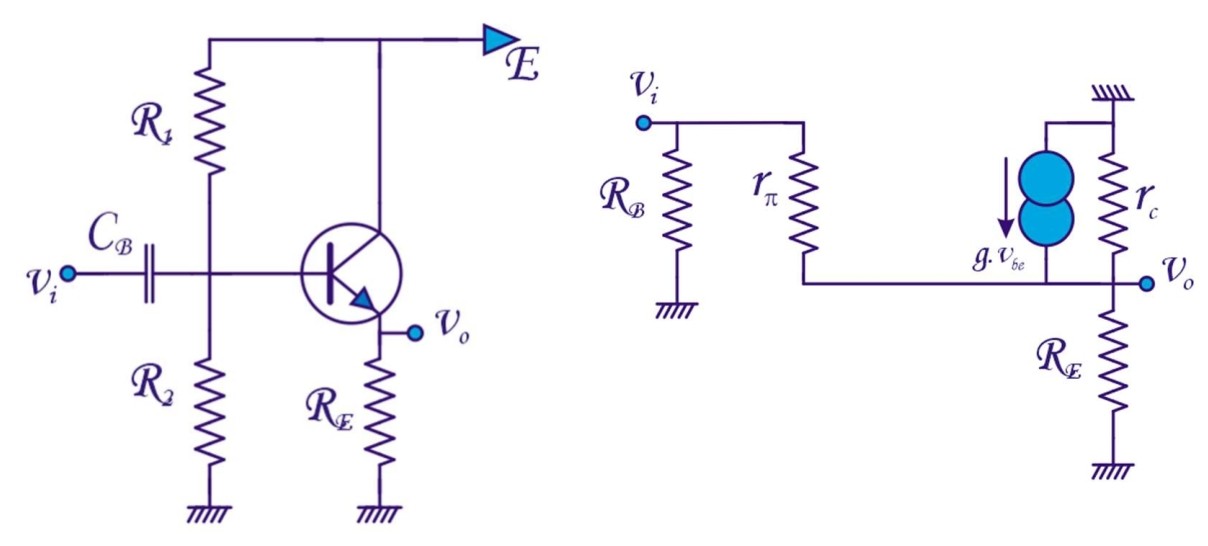
\includegraphics[width=14cm]{figures/ch02/amplifier9.jpg}
	\caption{CCA: circuit (left) and small-signal equivalent (right)}
	\label{fig:amplifier9}
\end{figure}

\begin{itemize}
	\item Voltage gain $A_v$: we see that $v_{be} = v_i - v_o$. In the output node, we can write:
	\begin{equation}
		\begin{split}
			v_o &= \frac{-g \; v_{be} + g_{\pi} v_i}{g_{\pi}  + g_c + G_E}\\
			&= \frac{-g \; (v_o - v_i) + g_{\pi} v_i}{g_{\pi}  + g_c + G_E}\\
			\rightarrow (g + g_{\pi}  + g_c + G_E) \; v_o &= (g + g_{\pi}) \; v_i\\
			\rightarrow  A_v = \frac{v_o}{v_i} &= \frac{g + g_{\pi}}{g + g_{\pi}  + g_c + G_E} \approx \frac{g}{g+G_E} \approx 1
		\end{split}
	\end{equation}
	\item Input impedance $Z_i$.\\
	Consider the circuit initially without $R_B$. Then
	\begin{equation}
		\begin{split}
			i_o &= g_\pi (v_i - v_o) \\
				&= g_\pi (1 - \frac{g + g_{\pi}}{g + g_{\pi}  + g_c + G_E}) v_i\\
				&= 	g_\pi (\frac{g_c + G_E}{g + g_{\pi}  + g_c + G_E}) v_i\\
				&\approx g_\pi \frac{G_E}{g} \\
			\rightarrow Z_i &= R_E \frac{g}{g_\pi} = \beta R_E
		\end{split}
	\end{equation}
	and thus $Z_i = \beta R_E \; || \; R_B$.
	\item Output impedance $Z_o$:
	$$i_o = (G_E + g_c + g_{\pi} + g)\; v_o$$
	and thus 
	$$Z_o = \frac{1}{G_E + g_c + g_{\pi} + g} \approx \frac{1}{g + G_E} \approx \frac{1}{g}$$
\end{itemize}

\subsection{Comparison of Topologies}
The characteristics of the different topologies - both for BJT as for the MOSFET (Common source, gate, and drain configurations) - are summarized in table \ref{table:comparison_amplifiers}. We only use intrinsic parameters of the transistors.

\begin{center}
	\begin{tabular}{||c | c | c | c||} 
		\hline
		& $Z_i$ & $Z_o$ & $|A_v|$ \\ [0.5ex] 
		\hline\hline
		CEA & $r_{\pi}$ & $r_c$ & $g\;r_c$ \\ 
		\hline
		CBA & $1/g$ & $r_c$ & $g\;r_c$ \\
		\hline
		CCA & $\beta R_E$ & $1/g$ & $1$ \\
		\hline
		CSA & $\infty$ & $r_{ds}$ & $g_m r_{ds}$ \\
		\hline
		CGA & $1/g_m$ & $r_{ds}$ & $g_m r_{ds}$ \\ 
		\hline
		CDA & $\infty$ & $1/g_m$ & $1$ \\ 
		\hline
	\end{tabular}
	\label{table:comparison_amplifiers}
\end{center}

\begin{minipage}{.5\textwidth}
	\centering
	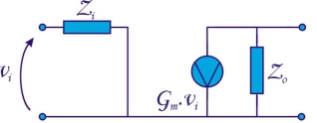
\includegraphics[width=6cm]{figures/ch02/amplifier10.jpg}
	\captionof{figure}{}
	\label{fig:amplifier10}
\end{minipage}%
\begin{minipage}{.5\textwidth}
	\centering
	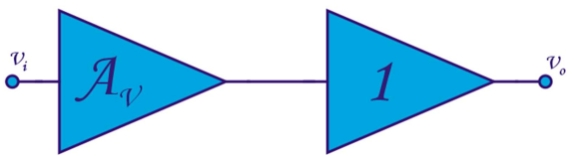
\includegraphics[width=5cm]{figures/ch02/amplifier11.jpg}
	\captionof{figure}{}
	\label{fig:amplifier11}
\end{minipage}
Figure \ref{fig:amplifier10}, the schematic representation of an amplifier as seen in chapter \ref{ch:introduction}, shows that as a general rule $|A_v| = g\;Z_o$. This can be verified in table \ref{table:comparison_amplifiers}. From this figure, we can also deduce that a good amplifier needs (a) a high input impedance to avoid drawing a large current from the previous stage and (b) a low output impedance to avoid making the output voltage depended on the impedance of the next stage. The only suitable configuration is the common collector (or CDA), but this amplifier has a gain of $\approx 1$. In conclusion, to implement a good amplifier we need a cascade of:
\begin{itemize}
	\item An amplifier with high gain, medium $Z_i$ and high $Z_o$,
	\item A buffer stage with gain $\approx 1$, high $Z_i$ and low $Z_o$, as in figure \ref{fig:amplifier11}.
\end{itemize}
Consequently, the gain will be high, and in- and output impedances will be as required.

\newpage
\section{Differential Amplifier}
\label{sec:diff_amplifier}
\subsection{Definition}
Until now, the amplifiers we studied only had a single input terminal and a single output terminal. We would like to create an amplifier that amplifies the \emph{difference} between two voltages. This can be useful to compare two signals as in an operational amplifier, or to remove the noise on two signals when this noise is significantly correlated (e.g. because it was created by the same noise source).
\begin{figure}[h!]
	\centering
	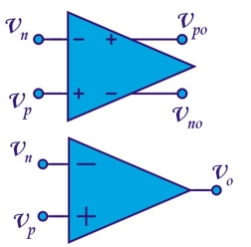
\includegraphics[width=5cm]{figures/ch02/diff_amp1.jpg}
	\caption{Differential amplifier with two (top) or one (bottom) output.}
	\label{fig:diff_amp1}
\end{figure}
There are $2$ inputs $v_p$ and $v_n$ (the positive and negative terminal). The goal is to amplify the difference $v_p - v_n$. This can be done with one or two outputs. In the latter case - also called the \emph{differential} case - the voltage between outputs $v_{po}$ and $v_{no}$ is:
$$
v_{os} = v_{po} - v_{no} = A_v \; (v_p - v_n)
$$
as in the top of figure \ref{fig:diff_amp1}. The other option is the single-output, asymmetrical amplifier:
$$
v_o = A_v \; (v_p - v_n)
$$
To make the analysis easier, we split the signal in two components:
\begin{itemize}
	\item A \emph{differential mode}: $v_d = v_p - v_n$,
	\item A \emph{common mode} $v_c = \frac{v_p + v_n}{2}$
\end{itemize}
This means that we can write $v_p = v_c + \frac{v_d}{2}$ and $v_n = v_c - \frac{v_d}{2}$. In a typical scenario, the common-mode signal can be a lot larger (order of magnitude several volts) than the differential mode (several milivolts).\\
With a single output, the output voltage is thus $v_o = A_d v_d + A_c v_c$:
\begin{itemize}
	\item The differential gain $A_d$, which is actually what we want, so it has to be as high as possible.
	\item The common mode gain $A_c$, which is a gain that we want to keep as low as possible - we want to reject the common mode. Ideally, it should be zero, but we will see that this is not possible (at least for a single-output amplifier).
\end{itemize}
We also define two so-called rejection ratios: the common-mode rejection ratio (CMRR) which is the ratio between $A_d$ and $A_c$: CMRR = $A_d/A_r$, and the power supply rejection ration PSRR, which expresses how variations in the power supply have an impact on the output. Both rejection ratios should be as high as possible, to remove unwanted, parasitic components in the output signal. They are typically expressed in decibel and in a good amplifier, are about $100$ - $120$ dB.\\
\subsection{Implementation}
The circuit to accomplish the requirements from the previous section, is shown in figure \ref{fig:diff_amp2}. We use two branches with identical npn transistors and identical collector resistances $R$. Both emitters are tied to a common node with voltage $v_e$. The bases of both transistors are the inputs. The outputs are measured at or between the collectors. The resistance $R_E$ carries a current $I_{RE}$.

\begin{figure}[h!]
	\centering
	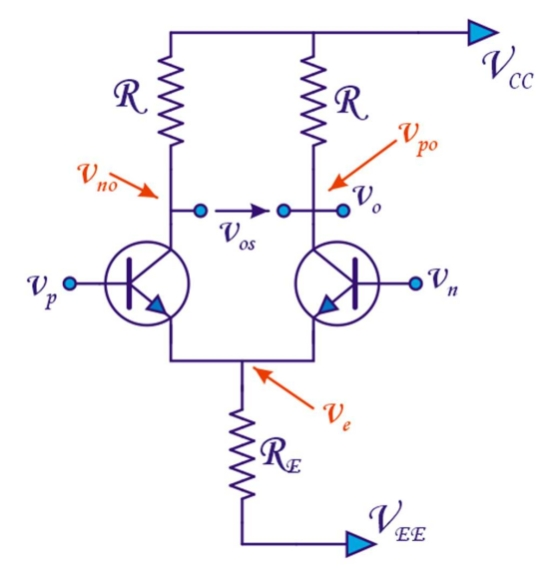
\includegraphics[width=8cm]{figures/ch02/diff_amp2.jpg}
	\caption{Structure of the differential amplifier}
	\label{fig:diff_amp2}
\end{figure}

\subsection{Common Mode}
If the input nodes $v_n$ and $v_p$ are at the same voltage, $v_n = v_p = v_c$, the two branches carry an identical current $I_{RE}/2$ and the  outputs $v_{no}$ and $v_{po}$ are both equal to $V_{CC} - R\;I_{RE}/2$. The differential output $v_{os}$ is than zero. Because of the symmetry in the circuit, this output is very robust and depends only on the differential signals. However, if there is some mismatch between both branches, e.g. the transistors or resistances are not completely identical, this is no longer the case.\\
When $v_n = v_p = v_c$, then $v_e = v_c - V_{BEQ} \approx v_c - 0.6$ V. The current in both branches is equal to $i_c = \frac{ I_{RE}}{2} = \frac{v_e - V_{EE}} {2R_E}$ and $v_{op} = v_{on} = v_o = V_{CC} - R \; i_c$. The symmetrical output $v_{os} = v_{po} -v_{po}$ is still zero, as it should be. The single output $v_o$ however, varies with $v_c$. This variation should be as small as possible.\\
To study the common-mode response, we can split the circuit into two parts. In a first stage, we split resistance $R_E$ into two parallel resistors of value $2R_E$, as in figure \ref{fig:diff_amp3}. Because of the symmetry and because both inputs are the same, there can be no current in the wire connecting both emitters, so we remove it. So, in effect, we can study both halves independently which means we only have to analyze the circuit in figure \ref{fig:diff_amp4}.

\begin{minipage}{.5\textwidth}
	\centering
	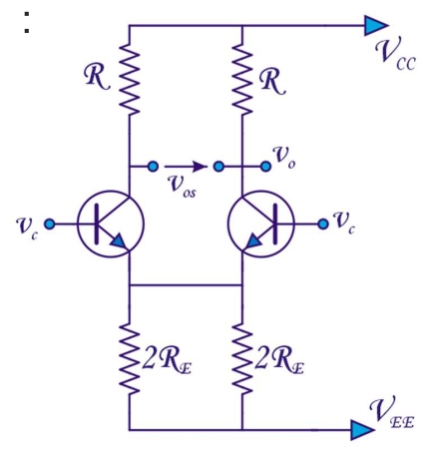
\includegraphics[width=6cm]{figures/ch02/diff_amp3.jpg}
	\captionof{figure}{}
	\label{fig:diff_amp3}
\end{minipage}%
\begin{minipage}{.5\textwidth}
	\centering
	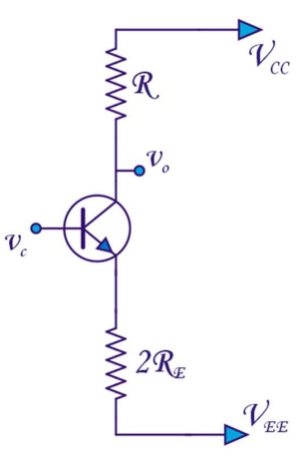
\includegraphics[width=4cm]{figures/ch02/diff_amp4.jpg}
	\captionof{figure}{}
	\label{fig:diff_amp4}
\end{minipage}

\subsection{Differential Mode}

With the common mode $v_c$ is zero, $v_p = + v_d/2$ and $v_n = -v_d/2$. This is a purely differential signal: if $v_p$ increases, $v_n$ would decrease with the same amount. To demonstrate that in this case $v_e = 0$ , we draw the small-signal equivalent circuit as in figure \ref{fig:diff_amp5} and use Millman's theorem to compute the voltage in $v_{on}$, $v_{op}$ and $v_e$. Note that $v_{be}$ in the left branch is $\frac{v_d}{2} - v_e$, and $-\frac{v_d}{2} - v_e$ in the right branch.

\begin{figure}[h!]
	\centering
	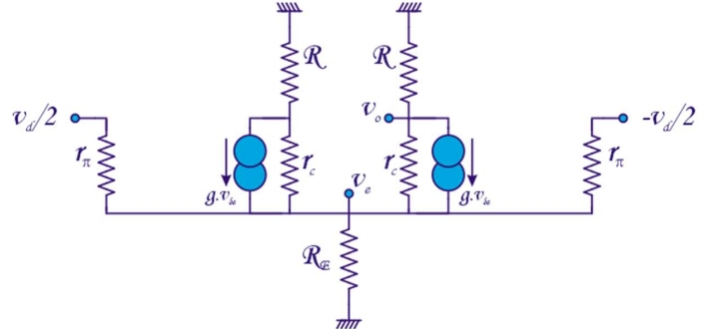
\includegraphics[width=12cm]{figures/ch02/diff_amp5.jpg}
	\caption{Differential mode: small-signal model}
	\label{fig:diff_amp5}
\end{figure}
\begin{align*}
	v_{po} &= \frac{g_c v_e - g(-\frac{v_d}{2} - v_e)}{G + g_c} \\
	v_{no} &= \frac{g_c v_e - g(\frac{v_d}{2} - v_e)}{G + g_c} \\
	v_e &= \frac{g_c v_{po} + g_c v_{no} + g(-\frac{v_d}{2} - v_e) + g(\frac{v_d}{2} - v_e) - g_{\pi} \frac{v_d}{2} + g_{\pi} \frac{v_d}{2}}{G_E + 2g_c + 2g_{\pi}}
\end{align*}
Substituting the expressions for $v_{on}$ and $v_{op}$ in the one for $v_e$ gives:
$$
v_e = \frac{g_c \frac{g_c v_e + g v_e}{g_c + G} + g_c \frac{g_c v_e + g v_e}{g_c + G} -g v_e -g v_e}{G_E + 2 g_c + 2 g_{\pi}}
$$
Because of the symmetries, all mentions of $v_d$ have disappeared in this expression. The solution is $v_e = 0$.\\
Building on the knowledge that $v_e = 0$ in a purely differential input signal (i.e. $v_E$ doesn't change when both $v_{op}$ and $v_{on}$ change with equal magnitude but opposite sign), we can draw the following circuit for the differential input of figure \ref{fig:diff_amp6}. In this circuit, the current through resistance $I_{RE}$ is constant because $v_E$ is constant for differential input signals. The collector current $I_{CQ}$ is constant and set by the common mode: $I_{CQ} = I_{RE}/2$. \\
Since we apply $+v_d/2$ to the left input, the current in the left loop increases by $i_c \approx g \; v_{be} = g \; v_d/2$ (remember: $v_e=0$). The current in the right loop decreases by the same amount:  $i_c \approx -g \; v_d/2$. So any additional current in the left loop flows in the right loop, keeping the current through $R_E$ constant, as established previously. The output voltages change as well: $v_{on} = -R \; g \; v_d/2$ and $v_{op} = +R \; g \; v_d/2$ and thus $v_{os} = g  \; R  \; v_d$.

\begin{minipage}{.5\textwidth}
	\centering
	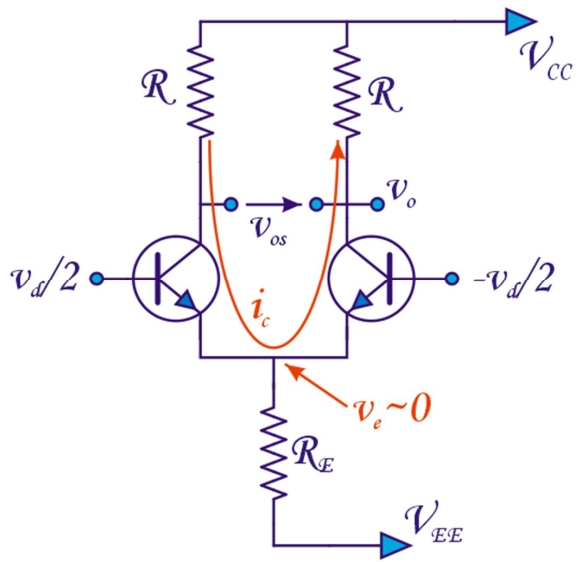
\includegraphics[width=7cm]{figures/ch02/diff_amp6.jpg}
	\captionof{figure}{}
	\label{fig:diff_amp6}
\end{minipage}%
\begin{minipage}{.5\textwidth}
	\centering
	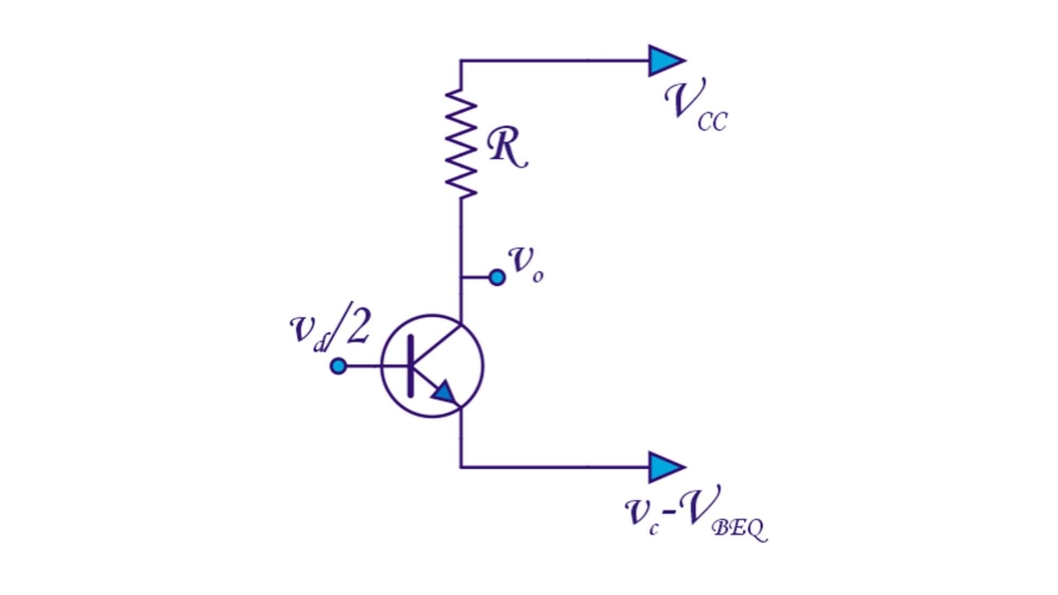
\includegraphics[width=9cm]{figures/ch02/diff_amp7.jpg}
	\captionof{figure}{}
	\label{fig:diff_amp7}
\end{minipage}

We can thus summarize that when we apply a differential signal, the emitter voltage $v_E$ stays fixed and equal to $\approx v_c - 0.6$ V and the circuit can be studied by considering only one branch, namely the one in figure \ref{fig:diff_amp7}.\\
This means we have an equivalent circuit to study the common mode in figure \ref{fig:diff_amp4} and a circuit to study the differential mode, in figure \ref{fig:diff_amp7}.

\subsection{Load-line Analysis}
The current $i_C$ is determined by the common mode, from figure \ref{fig:diff_amp4}:
\begin{equation}
	i_C = \frac{v_c - V_{BEQ} - V_{EE}}{2R_E}
\end{equation}
The load line equation is given by:
\begin{equation}
	V_{CC} - (v_c - V_{BEQ}) = R i_C + v_{CE}
\end{equation}
from figure \ref{fig:diff_amp7}.\\
The operating point $Q$ is found by the intersection of these two lines, as in figure \ref{fig:diff_amp8}. Note how $v_c$ impacts both lines: the current shifts up and down, and the load line moves parallel with varying $v_c$. This observation makes it very difficult to control the operating point. Commonly, the outer limits of $v_c$ are given, so an estimate of the range of $Q$ can be made.\\
As $v_d$ changes, one transistor moves up along the load line, while the other one moves down because the load line equation was derived from the circuit where we supposed the input was symmetrical around $v_c$.\\
\begin{figure}[h!]
	\centering
	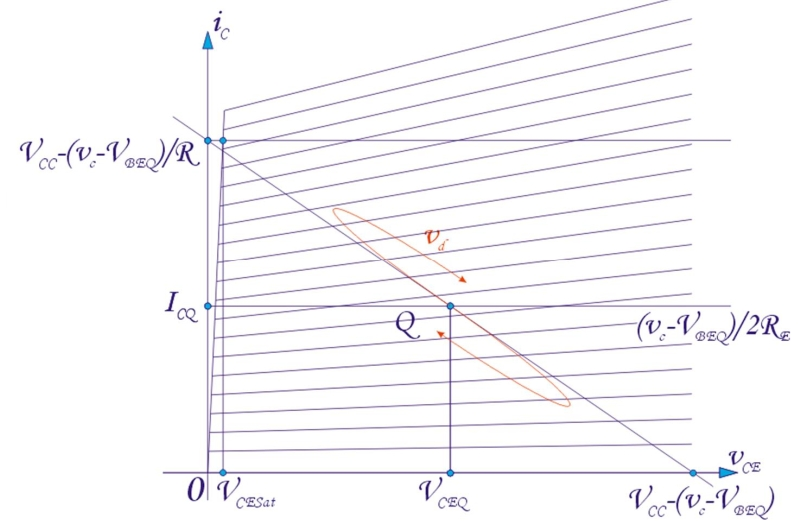
\includegraphics[width=12cm]{figures/ch02/diff_amp8.jpg}
	\caption{}
	\label{fig:diff_amp8}
\end{figure}

\subsection{Common \& Differential Gain}
The \emph{differential gain} $A_d$ can easily be computed by transforming the circuit in figure \ref{fig:diff_amp7} to its small-signal equivalent. The emitter voltage is an AC ground because this voltage doesn't change with $v_d$. The circuit is in fact a common-emitter amplifier. With $r_c$ in parallel with $R$ and $v_{be} = v_d/2$, we find:
\begin{equation}
	A_d = \frac{v_o}{v_d} = -\frac{g (R||r_c)}{2}
	\label{eq:differential_mode_gain}
\end{equation}
The \emph{common-mode gain} $A_c$ can be calculated by using the small-signal equivalent circuit for the circuit in figure \ref{fig:diff_amp4}. The result is found in figure \ref{fig:diff_amp9}. 

\begin{figure}[h!]
	\centering
	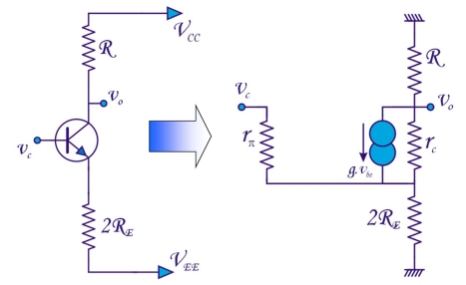
\includegraphics[width=10cm]{figures/ch02/diff_amp9.jpg}
	\caption{}
	\label{fig:diff_amp9}
\end{figure}
\begin{comment}
By applying Millman's theorem at emitter and collector, i.e. the output node:

\begin{itemize}
	\item $v_e = \frac{g_{\pi} v_c + g (v_c - v_e) + g_c v_o}{g_{\pi} + g_c + G_E/2}$
	\item $v_o = \frac{-g (v_c - v_e) + g_c v_e}{G + g_c} = \frac{-g}{G + g_c}v_c + \frac{(g + g_c)}{G + g_c}v_e$
\end{itemize}
Solving the first equation for $v_e$ gives:
\begin{equation}
	\begin{split}
		(g_{\pi} + g_c + G_E/2 + g) v_e &= g_{\pi} v_c + (g + g_c) v_o \\
		v_e &= \frac{g_{\pi} v_c + (g + g_c) v_o}{g_{\pi} + g_c + G_E/2 + g}
	\end{split}
\end{equation}
Substituting this in the expression for $v_o$ and solving for $v_o$ as function of $v_c$ gives:
\begin{equation}
	\begin{split}
		v_o = \frac{1}{G + g_c} (-g v_c + (g+g_c)  \frac{g_{\pi} v_c + (g + g_c) v_o}{g_{\pi} + g_c + G_E/2 + g})
	\end{split}
\end{equation}
\ldots Result:
\begin{equation}
	\begin{split}
		v_o = 
	\end{split}
\end{equation}
\end{comment}
This circuit is the same as the one in figure \ref{fig:amplifier4}, but with $2 R_E$ in stead of $R_E$. So we can reuse the result from equation \ref{eq:4resistor_dc}:

\begin{equation}
	\begin{split}
		A_c &= \frac{v_o}{v_c} = \frac{-g R r_c r_{\pi} + 2R R_E}{(r_c + R)(2R_E + r_{\pi}) + 2r_{\pi} R_E(1 + g r_c)} \\
		&\approx - \frac{R}{2R_E}
	\end{split}
	\label{eq:common_mode_gain}
\end{equation}
for a single output. For the differential output, $A_c = 0$.\\
From the results in equations \ref{eq:differential_mode_gain} and \ref{eq:common_mode_gain}, we find that:
\begin{equation}
	\begin{split}
	CMRR &= \frac{A_d}{A_c} \approx \frac{-\frac{g R}{2}}{- \frac{R}{2R_E}}\\
		 &\approx g \; R_E
	\end{split}
	\label{eq:cmrr}
\end{equation}
This means that is we want to increase the CMRR, we have to increase $R_E$. However, if we increase $R_E$, and since the voltage at the emitters is equal to $v_c - V_{BEQ}$, the current $I_{RE}$ through $R_E$ decreases. For each transistor, we have $I_{CQ} = I_{RE}/2$, and $g = \frac{I_{CQ}}{v_{th}}$. So each increase in $R_E$ will lead to a decrease in $I_{CQ}$ and thus also in a proportional decrease in $g$. Hence the CMRR will remain about the same.\\
A better way to increase $R_E$ is by using the circuit in figure \ref{fig:diff_amp10}, where we add an additional transistor between $R_E$ and $v_E$. We can explain the functioning as follows: with a fixed $V_{BB}$, the voltage at the emitter of the added transistor is $V_{BB} - V_{BEQ} = V_{BB} - 0.6$ V. This voltage is (relatively) fixed, and controls the current $I_{CQ}$ :
$$
I_{CQ} = \frac{1}{2}\frac{V_{BB} - V_{BEQ} - V_{EE}}{R_E}
$$
This current is fixed and doesn't depend (in a first approximation) on the collector voltage of the transistor (as long as this voltage is high enough). As the collector voltage can vary and the current remains constant, the collector sees a very large resistance.\\

\begin{minipage}{.4\textwidth}
	\centering
	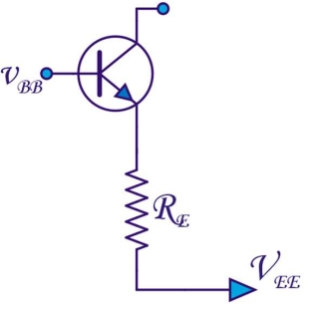
\includegraphics[width=5cm]{figures/ch02/diff_amp10.jpg}
	\captionof{figure}{}
	\label{fig:diff_amp10}
\end{minipage}%
\begin{minipage}{.5\textwidth}
	\centering
	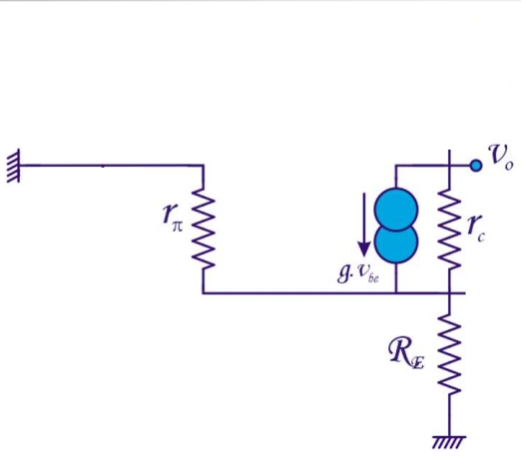
\includegraphics[width=7cm]{figures/ch02/diff_amp11.jpg}
	\captionof{figure}{}
	\label{fig:diff_amp11}
\end{minipage}

More formally, we can sketch the small-signal circuit as in figure \ref{fig:diff_amp11} and compute the output impedance as seen in  node $v_o$:
$$
	i_o = g_c (v_o - (-v_{be})) + g v_{be}
$$
Since $i_o$ also passes through the parallel combination of $R_E$ and $r_{\pi}$, we can state that:
$$i_o = -(G_E + g_{\pi}) v_{be}$$
and thus:
\begin{equation}
	\begin{split}
		i_o &= g_c v_o - (g + g_c) \frac{i_o} {G_E + g_{\pi}} \\
		(G_E + g_{\pi}) i_o &= (G_E + g_{\pi}) g_c v_o - (g + g_c) i_o \\
		(G_E + g_{\pi} + g + g_c) i_o &= (G_E + g_{\pi}) g_c v_o\\
		\Rightarrow Z_o = \frac{v_o}{i_o} &= \frac{G_E + g_{\pi} + g + g_c}{(G_E + g_{\pi}) g_c} \\
										   &\approx \frac{g}{g_c G_E} \\
		\Rightarrow Z_o &\approx (g r_c) \ R_E
	\end{split}
\end{equation}
The resistance $R_E$ is thus multiplied by the intrinsic transistor gain $gr_c \approx 1600$. The CMRR is thus $g (g r_c) R_E = g^2 r_c R_E$.

\subsection{Power-Supply Rejection Ratio}
To compute the power supply gain $A_{cc}$, we put the two inputs to AC ground an compute how $v_o$ varies if the power supply undergoes a voltage change $v_{cc}$. Using the small-signal equivalent circuit of figure \ref{fig:diff_amp7} with $v_d=0$, we find that $v_o = \frac{r_c}{r_c + R_C} v_{cc} \approx v_{cc}$ so the supply voltage variation is almost completely transferred to the output: $A_{cc} \approx 1$. The power supply rejection ratio PSRR is thus equal to $\bigg| \frac{A_d}{A_{cc}}  \bigg| \approx |A_d| \approx \frac{gR}{2}$.

\section{Operational Amplifier}
\label{sec:opamp}
An operational amplifier or \emph{OPAMP} is basically a differential amplifier with very high gain. It is typically constructed with a differential amplifier as input stage and an additional common-emitter stage to boost the gain of the differential amplifier. Schematically, we can see the internal structure of an OPAMP as in figure 
\ref{fig:opamp1} where there are $4$ stages:
\begin{enumerate}
	\item A single-output differential amplifier as input stage,
	\item A buffer stage to avoid that the next stage loads the output of the differential amplifier. This buffer stage has a high input impedance and low output impedance and a gain $A_v \approx 1$, like a common-collector amplifier.
	\item A high-gain stage, like a common-emitter amplifier,
	\item Another buffer stage to isolate the load circuitry from the OPAMP.
\end{enumerate}
\begin{figure}[h!]
	\centering
	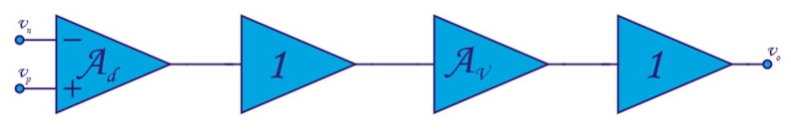
\includegraphics[width=14cm]{figures/ch02/opamp1.jpg}
	\caption{}
	\label{fig:opamp1}
\end{figure}
An OPAMP is very close to an ideal amplifier, which we will see in the next section. After that, we study the real OPAMP and see how non-idealities will impact its behavior.

\subsection{The Ideal Amplifier}
An OPAMP is represented by the symbol in figure \ref{fig:opamp2}. Just as the differential amplifier, it has two inputs, and the goal is to amplify the difference $v_i = v_p - v_n$, so that $v_o = A_v v_i$. Often, we define $v_i$ in the other sense ($v_i = v_n - v_p$) and assume $A_v$ is negative.
\begin{wrapfigure}{r}{0.4\textwidth}
	\centering
	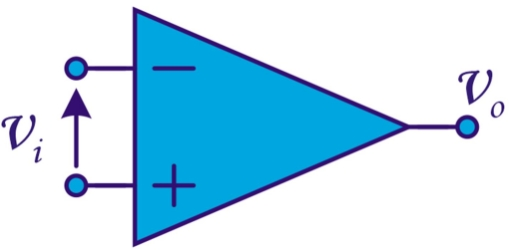
\includegraphics[width=5cm]{figures/ch02/opamp2.jpg}
	\caption{}
	\label{fig:opamp2}
\end{wrapfigure}
Ideally, the amplifier has these characteristics:
\begin{enumerate}
	\item The input impedance is infinite: $Z_i = \infty$. This means that currents $i^-$ and $i^+$ at the inputs are always zero.
	\item The output impedance is zero: $Z_o = 0$.
	\item The voltage gain is infinite: $A_v = \infty$.\footnote{In practice, the gain will really be very high: $\sim 100 000$.}
\end{enumerate}
An OPAMP is almost never used in isolation, because with such a high gain, the output will almost certainly be at the supply voltage. Most often an OPAMP is used with other elements that apply feedback from output to the input. The concept of feedback will be studied in more detail in chapter \ref{ch:feedback}.\\
Consider the topology in figure \ref{fig:opamp3}. The output of the OPAMP is fed back to the negative input terminal through resistance $R_2$ - this is called \emph{negative feedback}. The input $v_i$ is connected through resistance $R_1$ to the negative terminal of the OPAMP.

\begin{minipage}{.5\textwidth}
	\centering
	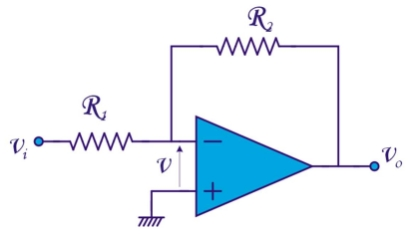
\includegraphics[width=6cm]{figures/ch02/opamp3.jpg}
	\captionof{figure}{}
	\label{fig:opamp3}
\end{minipage}%
\begin{minipage}{.5\textwidth}
	\centering
	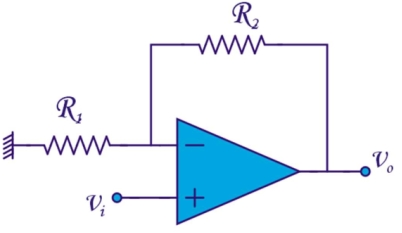
\includegraphics[width=6cm]{figures/ch02/opamp4.jpg}
	\captionof{figure}{}
	\label{fig:opamp4}
\end{minipage}
Voltage $v$ is found by considering that all current through $R_1$ also goes through $R_2$ because the input impedance of the OPAMP is infinite:
\begin{equation}
	\begin{split}
		\frac{v_i - v}{R_1} &= \frac{v - v_o}{R_2} \\
		\Rightarrow (R_1 + R_2) v &= R_2 v_i + R_1 v_o \\
		\Rightarrow v &= \frac{R_2 v_i + R_1 v_o}{R_1 + R_2}	
	\end{split}
\end{equation}
Output $v_o$ is equal to $A_v v$, so:
\begin{equation}
	\begin{split}
		v_o	&= -A_v v \\
			&= -A_v \frac{R_2 v_i + R_1 v_o}{R_1 + R_2}\\
	\Rightarrow	(R_1 + R_2) v_o	&= -A_v R_1 v_o - A_v R_2 v_i \\
	\Rightarrow v_o &= \frac{-A_v R_2}{R_1 + R_2 + A_v R_1} v_i \\
		&\approx -\frac{R_2}{R_1} v_i \text{ if } A_v \rightarrow \infty
	\end{split}
	\label{eq:opamp_gain1}
\end{equation}
Thus if $A_v$ is very high, the gain of this topology does not depend on the OPAMP gain and is set by the ratio of resistors $R_1$ and $R_2$: $A = -\frac{R_1}{R_2}$. Because the gain is negative, this topology is called the \emph{inverting amplifier}. The ratio $\frac{R_1}{R_2}$ can be set very precisely, and any temperature dependence disappears because both resistors vary in the same way with temperature. The gain $-\frac{R_2}{R_1}$ is the nominal gain $A_n$. Expression \ref{eq:opamp_gain1} can be rewritten as:
\begin{equation}
	\begin{split}
		\frac{v_o}{v_i} &= -\frac{A_n}{1 + \frac{A_n}{A_v} + \frac{1}{A_v}} = \frac{A_v A_n}{A_n + A_v + 1} \\
						&\approx -\frac{A_n}{1+\frac{A_n}{A_v}} 
	\end{split}
	\label{eq:opamp_gain2}
\end{equation}
This expression is valid for all feedback topologies.\\
We can also compute $\frac{v}{v_i}$:
\begin{equation}
	\begin{split}
		\frac{v}{v_i} &= \frac{v}{v_o} \frac{v_o}{v_i} \\
					  &= \frac{1}{A_v} \frac{-A_v R_2}{R_1 + R_2 + A_v R_1} \\
					  &\approx 0  \text{ if } A_v \rightarrow \infty
	\end{split}
\end{equation}
If $A_v \rightarrow \infty$, the voltage $v \rightarrow 0$. This does not mean we can short-circuit both input terminals, but this realization often simplifies analysis. This is why the negative input is called a \emph{virtual ground}.\\
For example, consider the circuit in \ref{fig:opamp4}, which is the same circuit as in \ref{fig:opamp3}, but with $v_i$ applied at the positive terminal. If $v \rightarrow 0$, the voltage at the negative input node is also $v_i$ and the current through $R_1$ is then equal to $\frac{v_i}{R_1}$. The same current flows through $R_2$: 
$$v_o - v_i = R_2 \frac{v_i}{R_1}$$
and consequently:
$$v_o = \big(1 + \frac{R_2}{R_1} \big) v_i$$
In figure \ref{fig:opamp3}, we had an amplifier with a negative gain; here, we obtain an amplifier with a positive gain (the \emph{non-inverting} amplifier).

\subsection{The Real Amplifier}
A real OPAMP, like the 741 OPAMP in figure \ref{fig:741_opamp} is far from ideal. The most important non-idealities are:

\begin{itemize}
	\item The input impedance is not infinite, hence $i^-, i^+ \ne 0$. For example, the base currents when bipolar transistors are the inputs of the differential amplifier as first stage.
	\item There is an offset current $i_d = i^+ - i^-$, when $v_o=0$. (typically $\sim 20 nA$). 
	\item Similarly, there is an offset voltage $e_d$ that's required to make $v_o = 0$. (typically $\sim mV$) as in figure \ref{fig:opamp10}. This also means that when $v_d \approx 0$, then $v_o \approx E_{supply}$.
	\begin{figure}[h!]
		\centering
		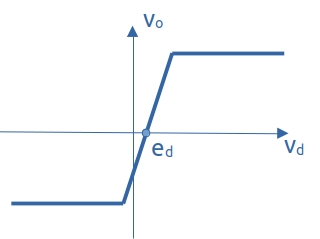
\includegraphics[width=8cm]{figures/ch02/opamp10.jpg}
		\caption{}
		\label{fig:opamp10}
	\end{figure}
	\item The voltage gain is not infinite: $A_v \ne \infty$. (typically around $100\;dB$ or $100000$)
	\item The bandwidth $\omega_0$ is limited.
	\item The slew rate and settling time. An OPAMP behaves as a two-pole system, so the output can not immediately follow the input. If we apply a step at the input, the output will increase but not immediately and will take some time to stabilize around the final value. These two effects are characterized by the slew rate and settling time, respectively.
\end{itemize}
\begin{minipage}{.5\textwidth}
	\centering
	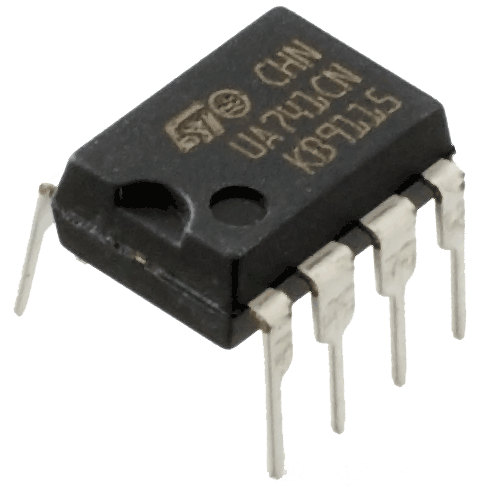
\includegraphics[width=5cm]{figures/ch02/741_opamp.png}
	\captionof{figure}{}
	\label{fig:741_opamp}
\end{minipage}%
\begin{minipage}{.5\textwidth}
	\centering
	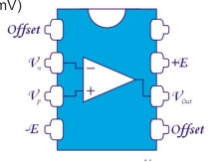
\includegraphics[width=5cm]{figures/ch02/opamp5.jpg}
	\captionof{figure}{}
	\label{fig:opamp5}
\end{minipage}
\\Furthermore, a real OPAMP requires a supply voltage $(+E, -E)$ and has a maximum allowed power consumption. The supply voltage can be symmetrical ($\pm 1.5V, \pm 5V, \pm 15V)$ or with the ground as reference ($+3.3V, +5V, +15V$).\\
Figure \ref{fig:opamp5} shows the typical pin configuration of a LM741 OPAMP, originally developed by Texas Instruments. Note the in -and output voltage $v_p$, $v_n$ and $v_o$, the supply voltages $+E$ and $-E$ and two offset pins to adjust offset currents and voltage.

\subsection{OPAMP Theory}
To model these non-ideal effects, we will use the OPAMP model in figure \ref{fig:opamp6}, including a non-zero output impedance $Z_o$.
\begin{figure}[h!]
	\centering
	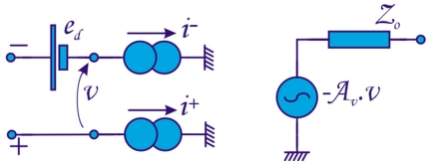
\includegraphics[width=9cm]{figures/ch02/opamp6.jpg}
	\caption{}
	\label{fig:opamp6}
\end{figure}
To demonstrate this, we study the effect of input bias currents and offset voltages when the OPAMP is used in the simple circuit of figure \ref{fig:opamp3}. Replacing the OPAMP by its model (with $Z_o = 0$) gives the equivalent circuit in figure \ref{fig:opamp7}.
\begin{figure}[h!]
	\centering
	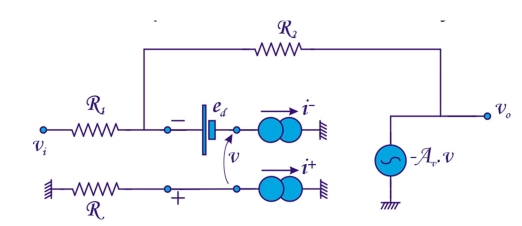
\includegraphics[width=12cm]{figures/ch02/opamp8.jpg}
	\caption{}
	\label{fig:opamp7}
\end{figure}
The idea to solve this problem is to consider all sources individually (with all other sources $=0$), and adding the results at the end. This is an application of the superposition principle. When we suppose $A_v \rightarrow \infty$:
\begin{itemize}
	\item $v_i$ : $v_0 = -\frac{R2}{R1} \; v_i$,
	\item $e_d$ : $v_o = \big(1 + \frac{R2}{R1} \big) \; e_d$, because this situation is as in figure \ref{fig:opamp4} with voltage $e_d$ at the negative input instead of $v_i$.
	\item $i^-$ : $v_o = R_2 \; i^-$ because with Millman:
	$$
	v = \frac{G_2 v_o - i^-}{G_1 + G_2}
	$$
	and since $v_o = -A_v v$, we rearrange and obtain:
	$$
	v_o = \frac{A_v}{G_1 + G_2 + A_v G2} i^- \approx R_2 \; i^-
	$$
	Another way to see this, is to realize there is no current through $R_1$: because $v=0$, both terminals of $R_1$ are at zero voltage. All current drawn by $i^-$ goes through $R_2$, thus $v_o - v = R_2 \; i^-$.
	\item $i^+$ : $v_o = -R \big(1 + \frac{R2}{R1} \big) \; i^+$ because a current $i^+$ generates a voltage $-R \; i^+$ at the positive terminal, replicating the situation of figure \ref{fig:opamp3};
\end{itemize}
The final expression is thus:
$$
v_o = -\frac{R_2}{R_1} v_i + \bigg(1 + \frac{R_2}{R_1} \bigg) \; e_d + R_2 \; i^- - R \bigg(1 + \frac{R_2}{R_1} \bigg) \; i^+
$$
We can draw these conclusions:
\begin{itemize}
	\item If $e_d$ is of the same order of magnitude as $v_i$, it will have a large impact on the output. The best way to take $e_d$ into account, is to first measure the output voltage without applying $v_i$. In this way, you measure $\big(1 + \frac{R2}{R1} \big) \; e_d$ and you subtract this value when you measure $v_o$ with $v_i$ at the input.
	\item The impact of $i^-$ can be reduced by choosing a small $R_2$. This is feasible because $A_n$ is the ratio of resistors; their actual value is of less importance.
	\item If you choose $R = R_1 || R_2$, then $R_2 \; i^- - R \bigg(1 + \frac{R2}{R1} \bigg) \; i^+ = R_2 (i^- - i^+)$ and you significantly reduce the impact of the input bias currents.
\end{itemize}
Since the gain is not infinite, a relative gain error $\epsilon$ will always be present. If we call the true gain of the OPAMP with feedback circuitry $A$, we know from equation \ref{eq:opamp_gain2} that:
\begin{equation}
A = \frac{v_o}{v_i}  \approx -\frac{A_n}{1+\frac{A_n}{A_v}} \approx -A_n
	\label{eq:nominal_gain}
\end{equation}
The relative gain error $\epsilon$ is thus:
\begin{equation}
	\begin{split}
	\epsilon &= \frac{A_n - A}{A_n} = \frac{A_n - \frac{A_n}{1+\frac{A_n}{A_v}}}{A_n}\\
			 &= 1 - \frac{1}{1+\frac{A_n}{A_v}} = 1-\frac{A_v}{A_v + A_n} \\
		     &= \frac{A_n}{A_v + A_n} \approx \frac{A_n}{A_v}
	\end{split}
	\label{eq:relative_gain_error}
\end{equation}
The gain error thus increases with increasing $A_n$ and with decreasing OPAMP gain (which happens at higher frequencies).

\subsubsection{The effect of feedback on the bandwidth}
In reality, the OPAMP has a limited bandwidth. We will model the OPAMP as a first-order system with a pole in $\omega = \omega_0$:
$$
A_v = \frac{A_{v0}}{1 + j \frac{\omega}{\omega_0}}
$$
This system has a cut-off frequency $f_0 = \omega_0 /  2\pi $.\\
Substituting this expression in equation \ref{eq:nominal_gain}, gives:
\begin{align*}
	A &\approx -\frac{A_n}{1+\frac{A_n}{A_v}}  & \text{ equation \ref{eq:nominal_gain}}\\
	  &= -\frac{A_n}{1+\frac{A_n}{A_{v0}}\big(1 + j \frac{\omega}{\omega_0}\big)}   & \text{ substitution }\\
	  &= -\frac{A_n}{\big(1 + \frac{A_n}{A_{v0}}\big) + j \frac{\omega}{\omega_0} \big(\frac{A_n}{A_{v0}}\big)} & \text{ rearrange real - imaginary parts }\\
	  &\approx -\frac{A_n}{\big(1 + \frac{A_n}{A_{v0}}\big)}  
	  \frac{1}{1 + j \frac{\omega}{\omega_0} \big(\frac{A_n}{A_{v0}}\big)} & \text{ because } \big(\frac{A_n}{A_{v0}}\big)^2 \text{ is very small }\\
	  &\approx - \frac{A_n}{1 + j \frac{\omega}{\omega_n}}
\end{align*}
where $\omega_n$ is a new cut-off frequency:
$$
\omega_n = \frac{A_{v0} \; \omega_0}{A_n}
$$
This means that by using the OPAMP with the feedback circuitry, the gain has decreased and becomes $A_n$, but the bandwidth (the cut-off frequency) has increased. What remains constant is the \emph{gain-bandwidth product} $GBW$:
$$
A_n \times \omega_n = A_{v0} \times \omega_0 = GBW
$$
Figure \ref{fig:opamp11} represents the Bode curve of the OPAMP self (in blue), with a cut-off at $\omega_0$ and DC-gain $A_{v0}$, and the OPAMP with feedback circuitry (in green). The latter curve has a lower DC-gain $A_n$, but a larger bandwidth $\omega_n$. Another issue is also highlighted in the graph: if the frequency increases, the gain decreases and the relative gain error increases. If a maximum $\epsilon$ is imposed, the signal frequency cannot go beyond $\omega_{max}$.
\begin{figure}[h!]
	\centering
	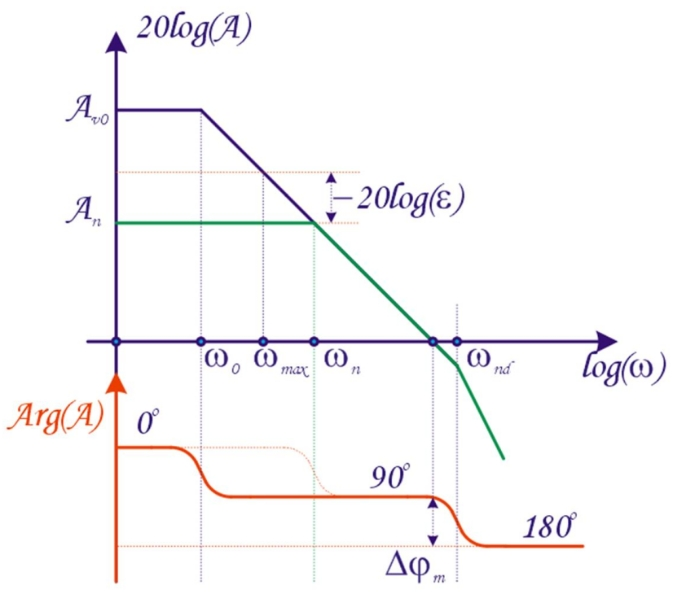
\includegraphics[width=10cm]{figures/ch02/opamp11.jpg}
	\caption{}
	\label{fig:opamp11}
\end{figure}


\subsubsection{Summary}
When an OPAMP is used for data acquisition (which is often the case), lots of errors will be introduced:
\begin{itemize}
	\item due to an offset voltage $e_d$,
	\item due to a differential input current $i_d$,
	\item due to the limited gain $A_v < \infty$, which results in a relative gain error $\epsilon$,
	\item due to the limited bandwidth $\omega_0$
\end{itemize}
You'll have to take all these errors into account, or avoid them by e.g. using OPAMPs with a low offset. In any case, because an OPAMP is inherently a second-order system, we have to live with a delay during acquisition, due to a non-zero settling time.
\subsection{Unity Gain Buffer}
\label{sec:unity_gain_buffer}

A commonly used OPAMP configuration is the one in figure \ref{fig:unity_gain}, where the output node is directly connected to the negative input terminal. With $v$ equal to zero, we immediately see that $v_o = v_i$, or that $A_n = 1$. We use the equivalent model in figure \ref{fig:unity_gain_small_signal} to study the different parameters more formally.\\
\begin{minipage}{.4\textwidth}
	\centering
	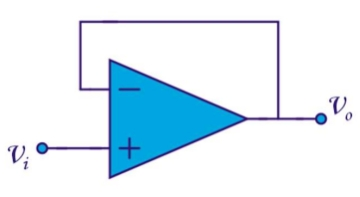
\includegraphics[width=6cm]{figures/app/opamp_ex2.jpg}
	\captionof{figure}{}
	\label{fig:unity_gain}
\end{minipage}%
\begin{minipage}{.6\textwidth}
	\centering
	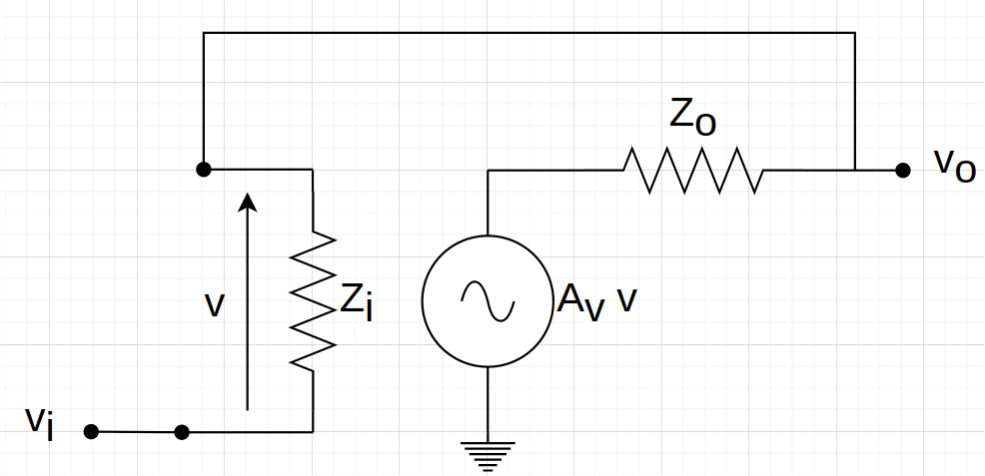
\includegraphics[width=8cm]{figures/app/opamp_ex3b.jpg}
	\captionof{figure}{}
	\label{fig:unity_gain_small_signal}
\end{minipage}
\begin{enumerate}
	\item Voltage gain $A_v$:
	\begin{align*}
		v_o &= \frac{G_o (- A_v v) + G_i v_i}{G_o + G_i} \\
			&= \frac{G_o A_v (v_i - v_o) + G_i v_i}{G_o + G_i} \\
		%\rightarrow (G_o + G_i +A_v G_o) \; v_o &= (G_i + A_v G_o) \; v_i \\
		\rightarrow \frac{v_o}{v_i} &= \frac{G_i + A_v G_o}{G_o + G_i +A_v G_o} \\
			&\approx \frac{A_v G_o}{A_v G_o} = 1\\
	\end{align*}
	\item Input impedance $Z_i$:
	\begin{align*}
		i_i &= G_i (v_i - v_o) \\
			&= G_i (1 - \frac{G_i + A_v G_o}{G_o + G_i +A_v G_o}) v_i \\
			&= G_i \frac{G_o}{G_o + G_i +A_v G_o} v_i \\
			&\approx \frac{G_i}{A_v} v_i \\
		\rightarrow Z_i = \frac{v_i}{i_i}&= A_v \; Z_i
	\end{align*}
	\item Output impedance $Z_o$:
	\begin{align*}
		i_o &= G_i v_o + G_o (v_o - (- A_v v)) \\
			&= ( G_i + (1 + A_v) G_o ) v_o \\
			&\approx A_v G_o v_o \\
		\rightarrow Z_o = \frac{v_o}{i_o} &= \frac{Z_o}{A_v}
	\end{align*}
\end{enumerate}
So this circuit has unity gain, a very high input impedance $A_v Z_i$ and a very low output impedance $\frac{Z_o}{A_v}$. In summary, it is the ideal buffer to isolate one stage from the next.\\
%Appendix \ref{app:opamp_examples} contains more OPAMP examples.